\documentclass{article}

\usepackage[shellescape]{gmp}
\usepackage[utf8]{inputenc}
\usepackage{german}

\usepackage{geometry}
\geometry{margin=2cm, left=2.2cm}

\usepackage{graphicx}
\DeclareGraphicsRule{*}{mps}{*}{}

\usepackage{pdflscape}

\usepackage{titling}
\setlength{\droptitle}{80px}

\usepackage{listings}
\usepackage{xcolor}
\usepackage{courier}

\usepackage[colorlinks=true,urlcolor=blue]{hyperref}
\usepackage{soul}

\renewcommand{\figurename}{Abbildung}
\begin{document}
\title{\Large Einsendeaufgabe \\ OOD}
\author{\normalsize Stefan Berger}
\date{}
\maketitle

\pagebreak

\section{Anwendungsfälle}
\paragraph{}
Das folgende Anwendungsfalldiagramm ersetzt das bisherige, das in einem früheren Stadium des Entwurfsprozesses entstanden war.
\vspace{50px}
\begin{figure}[h]
\centering
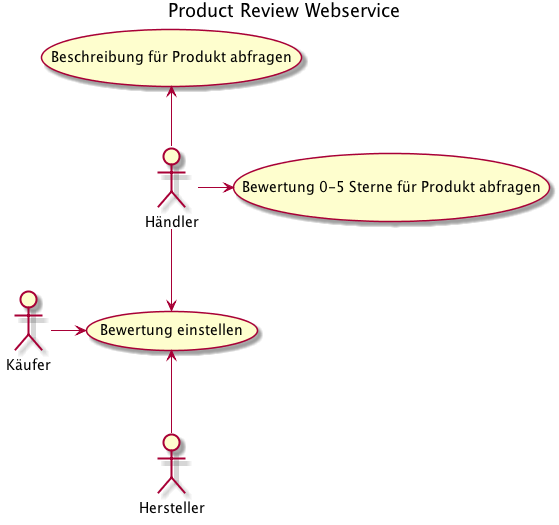
\includegraphics{mps/usecase.1}
\caption{Anwendungsfalldiagramm}
\end{figure}

\pagebreak

\begin{landscape}
\section{Komponenten und Klassen}
Das Komponnenten- und das Klassendiagramm wurden auch aktualisiert.
\vspace{50px}
\begin{figure}[h]
\centering
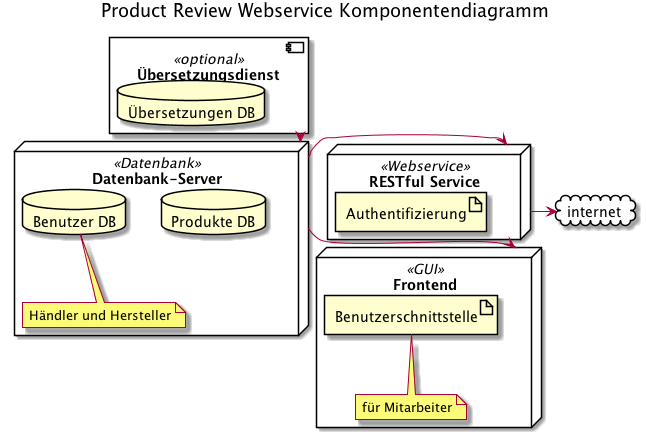
\includegraphics{mps/component.1}
\caption{Komponentendiagramm des Webservice}
\end{figure}

\pagebreak

\begin{figure}[h]
  \centering
  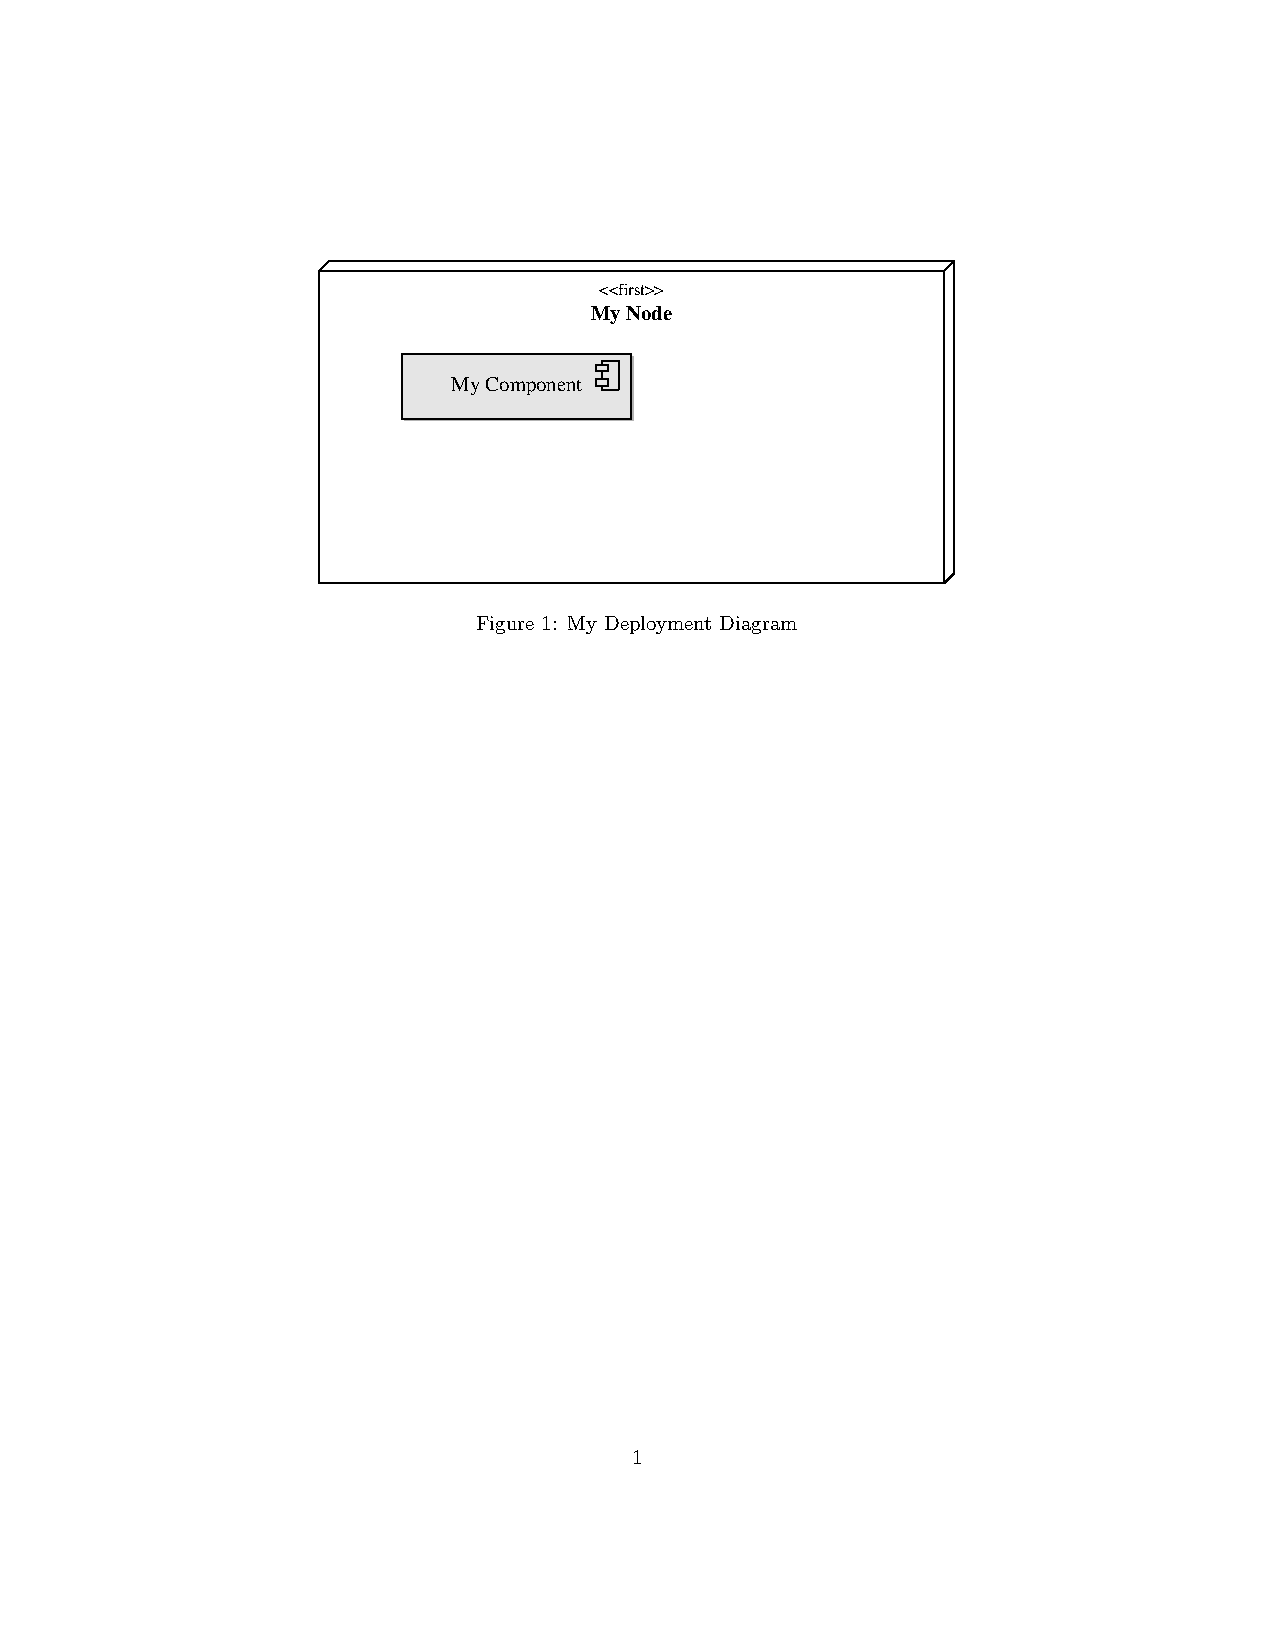
\includegraphics{mps/class.1}
  \caption{Klassendiagramm des Webservices}
\end{figure}

\end{landscape}

\section{Spike}
\paragraph{}
Den Kunden soll ein HTML-Snippet zur Verfügung gestellt werden. Dafür ist ein Prototyp erstellt worden. Bei der Erstellung wurde darauf geachtet, dass das HTML in den verschiedensten Endanwendungen zum Einsatz kommen kann. Insbesondere soll es nur wenige Zeilen umfassen und wenig Bandbreite benötigen. Es soll außerdem
\begin{itemize}
  \item wiederverwendbar
  \item einfach zu implementieren
  \item dokumentiert
  \item flexibel und
  \item durch CSS anpassbar
\end{itemize}
sein.

\paragraph{}
Im HEAD-Element der Webseite sind drei Dateien einzubinden:
\lstdefinelanguage{JavaScript}{
  keywords={typeof, new, true, false, catch, function, return, null, catch, switch, var, if, in, while, do, else, case, break},
  keywordstyle=\color{blue!67}\bfseries\itshape\ttfamily,
  ndkeywords={class, export, boolean, throw, implements, import, this},
  ndkeywordstyle=\color{darkgray}\bfseries,
  identifierstyle=\color{black!67},
  sensitive=false,
  comment=[l]{//},
  morecomment=[s]{/*}{*/},
  commentstyle=\color{purple}\ttfamily,
  stringstyle=\color{black}\ttfamily\itshape,
  morestring=[b]',
  morestring=[b]",
  emph={script, div, id, src, link, rel, href},
  emphstyle=\color{blue!50},
  backgroundcolor=\color{lightgray!20},
  linewidth=18cm,
  numberstyle=\color{lightgray},
  framexleftmargin=22px,
  xleftmargin=.2\textwidth, xrightmargin=.2\textwidth
}
\begin{lstlisting}[language=JavaScript,numbers=left,caption={Verweise im HTML-HEAD},captionpos=b]
<link rel="stylesheet" href="font-awesome.min.css">
<link rel="stylesheet" href="styles.css">
<script src="jquery-3.3.1.min.js"></script>
\end{lstlisting}

\paragraph{}
Eine Beispielimplementierung der Liste mit Produktreviews besteht aus genau 10 Zeilen, in denen unter anderem eine zusätzliche JavaScript-Datei geladen wird:

\begin{lstlisting}[language=JavaScript,numbers=left,caption={Das einzufügende Snippet},captionpos=b]
<script>
function getFilter(){
  return {
    field: "product",
    value: "p1"
  }
}
</script>
<div id="container"></div>
<script src="snippet.js"></script>
\end{lstlisting}

Die Zeilen 4 und 5 sind vom Kunden anzupassen. In dem Feld \texttt{value} muss die SKU des Produkts angegeben werden, dessen Reviews ausgegeben werden sollen.

\paragraph{}
Die CSS-Datei besteht ebenfalls aus wenigen Zeilen:
\lstdefinelanguage{css}{
  keywords={color, width, border, margin, bottom},
  keywordstyle=\color{blue},
  ndkeywords={px},
  ndkeywordstyle=\color{blue},
  identifierstyle=\color{black!67}\itshape\ttfamily,
  sensitive=false,
  comment=[l]{\#},
  morecomment=[s]{.}{\ },
  commentstyle=\color{black!67}\itshape\ttfamily,
  stringstyle=\color{gray}\ttfamily\itshape,
  morestring=[b]',
  morestring=[b]",
  backgroundcolor=\color{lightgray!20},
  linewidth=18cm,
  numberstyle=\color{lightgray},
  framexleftmargin=22px,
  xleftmargin=.2\textwidth, xrightmargin=.2\textwidth
}
\begin{lstlisting}[language=css,numbers=left,caption={Das CSS des Snippets},captionpos=b]
.checked {
  color: #FFD700;
}

.unchecked {
  color: gray;
}

.review {
  width: 400px;
  border: 1px solid lightgray;
  margin: 20px;
}
\end{lstlisting}

\paragraph{}
Die Spike-Lösung ist auf \href{http://s-berger-bmio.bplaced.net/4/SWT/OOD/}{\ul{http://s-berger-bmio.bplaced.net/4/SWT/OOD/}} zu finden.

\end{document}
